\documentclass[9pt,lineno]{elife}
\usepackage{fullpage,amsmath,url,cases}
\usepackage{natbib,longtable,graphicx,tikz}
%\usepackage{subfig}
\usepackage{url}
%\@ifundefined{showcaptionsetup}{}{%
%\PassOptionsToPackage{caption=false}{subfig}}
\graphicspath{{./figures/}{./figures/otherFigures/}}
\usepackage{xcolor}
\usepackage{colortbl}
\definecolor{RubineRed}{RGB}{240, 0, 240}       % RubineRed  Approximate PANTONE RUBINE-RED
%\usepackage{subfig}
\usepackage{listings}
\usepackage{color}

%%%%%%%%%%%%%%%%%%%%%%%%%%%%%%%%%% referencing %%%%%%%%%%%%%%%%%%%%%%%%%%%%%%%%%%
\usepackage{natbib}
\usepackage{hyperref}
\usepackage{xcolor}
\hypersetup{
    colorlinks,
    %linkcolor={red!50!black},
    linkcolor={black},
    citecolor={blue!50!black},
    urlcolor={blue!80!black}
}

%%%%%%%%%%%%%%%%%%%%%%%%%%%%%%%%%%%%%%%%%%%%%%%%%%%%%%%%%%%%%%%%%%%%%%%%%%%%%%%%
\usepackage[colorinlistoftodos]{todonotes}
%\usepackage[disable]{todonotes}

\usepackage{placeins}
\usepackage{flafter}

\newcounter{todocounter}
\newcommand{\todonum}[2][]
{\stepcounter{todocounter}\todo[#1]{\thetodocounter: #2}}

\newcommand{\done}[2][]
{\todo[color=green!40, #1]{#2}}

\newcommand{\donenum}[2][]
{\stepcounter{todocounter}\done[#1]{\thetodocounter: #2}}
%%%%%%%%%%%%%%%%%%%%%%%%%%%%%%%%%%%%%%%%%%%%%%%%%%%%%%%%%%%%%%%%%%%%%%%%%%%%%%%%

\definecolor{dkgreen}{rgb}{0,0.6,0}
\definecolor{gray}{rgb}{0.5,0.5,0.5}
\definecolor{mauve}{rgb}{0.58,0,0.82}

\lstset{frame=tb,
  language=Java,
  aboveskip=3mm,
  belowskip=3mm,
  showstringspaces=false,
  columns=flexible,
  basicstyle={\small\ttfamily},
  numbers=none,
  numberstyle=\tiny\color{gray},
  keywordstyle=\color{blue},
  commentstyle=\color{dkgreen},
  stringstyle=\color{mauve},
  breaklines=true,
  breakatwhitespace=true,
  tabsize=3
}
\lstset{language=bash}


\title{Supplementary Material I}
\author{Sha Joe Zhu, Jacob Almagro-Garcia, Jason Hendry and Gil McVean}
\date{}

\usepackage[label font=bf,labelformat=simple, position = top, justification=RaggedRight,singlelinecheck=false]{subfig}
\renewcommand{\thesubfigure}{\Alph{subfigure}}

\setcounter{equation}{0}
\setcounter{figure}{0}
\setcounter{table}{0}
\setcounter{page}{1}
\makeatletter
\renewcommand{\thesection}{S1}
\renewcommand{\theequation}{S1.\arabic{equation}}
\renewcommand{\thefigure}{S1.\arabic{figure}}
\renewcommand{\thetable}{S1.\arabic{table}}
\renewcommand{\bibnumfmt}[1]{[S1#1]}
\renewcommand{\citenumfont}[1]{S1#1}
%%%%%%%%%% Prefix a "S" to all equations, figures, tables and reset the counter %%%%%%%%%%

%\floatsetup[figure]{style=plain,subcapbesideposition=top}
%\newsubfloat{figure}



%%%%%%% Start on new page
\renewcommand{\thepage}{S1-\arabic{page}}
\begin{document}
\maketitle{}
%\listoftodos
%\clearpage
%\setcounter{page}{1}

%\maketitle
\tableofcontents

%\setcounter{section}{0}

\newpage




\section{Deconvolution in the presence of IBD}



%\todo{expand methods}

%\subsection{Deconvolution of mixed infection}

\subsection{Notations}
We use the same notations as \citet{Zhu2017} (see Table~\ref{tab:notation}). Our data, $D$, are the allele read counts of sample $j$ at a given site $i$, denoted as $r_{j,i}$ and $a_{j,i}$ for reference (REF) and alternative (ALT) alleles respectively.  These are assigned values of $0$ and $1$ respectively. Here we consider only bi-allelic loci, though future extension to include multi-allelic sites is simple.  The empirical allele frequencies within a sample (WSAF) $p_{j,i}$ and at population level (PLAF) $f_i$ are calculated by $ \frac{a_{j,i}}{a_{j,i} + r_{j,i}}$ and $ \frac{\sum_j a_{j,i}}{\sum_j a_{j,i} + \sum_j r_{j,i}}$ respectively. Since all data in this section refers to the same sample, we drop the subscript $j$ from now on.

\begin{table}[htb]\centering
\begin{tabular}{c|c}\hline
$i$              & Marker index\\
$j$              & Sample index \\
$r$              & Read count for reference allele \\
$a$              & Read count for alternative allele \\
$f$              & Population level allele frequency (PLAF) \\
$n$              & Number of strains within sample \\
$l$              & Sequence length \\
$\mathbf{w}$      & Proportions of strains \\
%$\mathbf{x}$	& Log titre of strains \\
$\mathbf{h}_{i}$ & Allelic states of $n$ parasite strains at site $i$ \\
$h_{k,i}$   & Allelic state of parasite strain $k$ at site $i$\\
$p$              & Observed within sample allele frequency (WSAF) \\
$q$              & Unadjusted expected WSAF  \\
$\pi$            & Adjusted expected WSAF \\
%$\Xi$            & Reference panel\\
%$\xi_{k,i}$     & Allelic state of reference panel strain $k$ at site $i$\\
%$G$              & Scaling factor used for genetic map\\
$e$              & Probability of read error\\
$\mathcal{S}_{i}$ & IBD state at site $i$ \\
$\mathcal{G}$ & genotype state at site $i$ \\
\hline
\end{tabular}
\vspace{.2cm}
\caption{Table summarising the notation used in this article.}\label{tab:notation}
\end{table}

\subsection{Model with the IBD state}

We describe the mixed infection problem by considering the number of strains, $n$, the relative abundance of each strain, $\mathbf{w}$, and their allelic states, $\mathbf{h}_{i}$. In addition to \citet{Zhu2017}, we also infer the IBD-state $\mathcal{S}_{i}$, which describes the strain relationships at each site $i$. For example, for three strains, the IBD-state could be one of the five cases: (1) all strains are not IBD; (2)(3)(4) only two strains are IBD; (5) all strains are IBD (see Table~\ref{tab:encode}). To simplify our problem, we assume independence between each marker, and drop the subscript $i$ from now on. Similar to \citet{Jack2016}, we use a Bayesian approach and define the posterior probabilities of $n$, $\mathbf{w}$, $\mathbf{h}$ and $\mathcal{S}$,  as:

\begin{equation}
P(n, \mathbf{w}, \mathbf{h}, \mathcal{S}| e, D) \propto L(n, \mathbf{w}, \mathbf{h}, \mathcal{S} | e, D) \times P(n, \mathbf{w}, \mathbf{h}, \mathcal{S}), \label{eqn:post}
\end{equation}
where $e$ is the read error rate.

\begin{table}
\centering
\begin{tabular}{c|ccc}
  Index / & \multicolumn{3}{c}{IBD state} \\
viterbi state    & k = 2& k = 3 & k = 4 \\ \hline
1	  &1-2	&	1-2-3	&1-2-3-4	\\
2	  &2-2	&	2-2-3	&2-2-3-4	\\
3	  &	  	&	3-2-3	&3-2-3-4	\\
4	  &		  &	1-3-3	&4-2-3-4	\\
5	  &		  &	3-3-3	&1-3-3-4	\\
6	  &	  	&		    &3-3-3-4	\\
7	  &	  	&		    &4-3-3-4	\\
8	  &	  	&	    	&1-4-3-4	\\
9	  &	  	&		    &4-4-3-4	\\
10	&	  	&		    &3-4-3-4	\\
11	&	  	&		    &1-2-4-4	\\
12	&		  &		    &2-2-4-4	\\
13	&	  	&		    &4-2-4-4	\\
14	&	  	&	    	&1-4-4-4	\\
15	&	  	&		    &4-4-4-4	\\
\end{tabular}
\caption{IBD configurations of number of strains are 2, 3 and 4. The state 1-2 denotes that strains 1 and 2 are non-IBD; The state 2-2 denotes that strain 1 is IBD with strain 2. The state 2-2-3 denotes that strain 1 is IBD with strain 2, but not strain 3. }\label{tab:encode}
\end{table}


\noindent We assume a prior in which the haplotypes of the $n$ strains are independent of each other and dependent only on the IBD state. Let $\mathcal{G}$ be the genotype state that is derived from the IBD state $\mathcal{S}$. We assume uniform prior on $\mathcal{G}|\mathcal{S}$. For example, if $n=3$ and only strains 1 and 2 are IBD, the genotype state at site $i$ $\mathcal{G}$ could be $\{0,0,0\}$; $\{0,0,1\}$; $\{1,1,0\}$ and $\{1,1,1\}$. Therefore, we can decompose the joint prior as:
\begin{equation}
P(n, \mathbf{w}, \mathbf{h}, \mathcal{S}) = P(n) \times P(\mathbf{w}|n) \times P(\mathbf{h} , \mathcal{S}|n),
\end{equation}
where
\begin{equation}
P(\mathbf{h}, \mathcal{S}|n) = P(\mathcal{S}|n) \times \sum_{\xi \in \mathcal{G}} P(\mathbf{h} | \xi) \times P(\xi|\mathcal{S}).
\label{eqn:}
\end{equation}

\noindent For details of the likelihood and the prior on the proportions see \citet{Zhu2017} sections 2.2.1 and 2.2.2. We use the following expression for the expected WSAF $q$, as:
\begin{equation}
q = \mathbf{w}\cdot\mathbf{h}.\label{eqn:qij_full_sum}
\end{equation}



\noindent The data, which can be summarised by the reference and alternative allele read counts at each site, is modelled through a beta-binomial distribution given the expected WSAF.  We model the data at distinct segregating sites as independent.  Thus the likelihood function  in Eqn.~\eqref{eqn:post} is only dependent on the haplotypes present and their frequencies through their contribution to $q_{i}$.

%; i.e. $L(n, \mathbf{w}, \mathbf{h}, | \Xi, e, D) = \prod_{i=1}^l L(q_i | \Xi, e, D)$.

To incorporate sequencing error, we modify the expected WSAF such that the allele frequency of `REF' read as `ALT' is $(1 - q_i)e$, and the allele frequency of `ALT' read as `REF' is $q_ie$. Thus, the adjusted expected WSAF becomes:

\begin{equation}
\pi_i = q_i + (1 - q_i)e - q_ie = q_i + (1 - 2q_i)e.\label{eqn:adj_q}
\end{equation}

\noindent We model over-dispersion in read counts relative to the Binomial using a Beta-binomial distribution. Specifically, the read counts of `ALT' are identically and independently distributed (i.i.d.) Bernoulli random variables with probability of success $v_i$; i.e. $a_i \sim Binom(a_i + r_i, v_i)$, and $v_i \sim Beta(\alpha, \beta)$, where $E(v_i) = \alpha/(\alpha+\beta) = \pi_{i}$. This is achieved by setting $\alpha = c\cdot \pi_{i} $ and $\beta = c\cdot (1-\pi_{i})$, such that the variance of the WSAF is inversley proportion to $c$.  Combined, we have:

\begin{equation}
L(q_{i}| e, D) \propto \frac{\Gamma(a_i + c\cdot \pi_{i}) \Gamma(r_i + c\cdot (1-\pi_{i}))}{\Gamma(c\cdot \pi_{i})\Gamma(c\cdot (1-\pi_{i}))}. \label{eqn:llk}
\end{equation}


%\subsubsection{Metropolis-Hastings update for proportions}\label{sec:updateP}
%\todo{To keep this? or just mention this is the same as \citet{Zhu2017}}
%We update $\mathbf{w}|n$, through the underlying log titres, $\mathbf{x}|n$. Specifically, we choose $i$ uniformly from $n$ and propose new $x_i'$s from $x_i' = x_i + \delta x$, where $\delta x \sim N(0, \sigma^2/s)$, and $s$ is a scaling factor. The new proposed proportion is therefore $\frac{\exp(x_k')}{\sum_{k=1}^n \exp(x_k')}$. Since the proposal distribution is symmetrical, the Hastings ratio is 1. A new update is accepted with probability

 %$$\min\left(1, \frac{P(\mathbf{w}'|n)}{P(\mathbf{w}|n)} \frac{L(\mathbf{w}', \mathbf{h}, {\mathcal S} | e, D)}{L(\mathbf{w}, \mathbf{h}, {\mathcal S} | e, D)}\right).$$

%\subsubsection{Gibbs sampling for haplotype and IBD-configuration update}


%\paragraph{Prior on $\mathcal{S}|n$}

%Inbreeding coefficient.


%To perform inference about the haplotypes present and their proportions we use Markov chain Monte Carlo (MCMC). We use a Metropolis-Hastings algorithm to sample proportions ($\mathbf w$) given $\mathbf h$; and use a Gibbs sampler to update $\mathbf h$ for a given $\mathbf w$, with two types of update: a single haplotype and a pair of haplotypes.

%\begin{itemize}
  %\item Likelihood
  %\item MCMC
%\end{itemize}

%Hidden markov model, $\mathcal{S}_{i}$ transition probability $t_{i, i+1}$, and emission probability $P(\mathbf{h} | \xi)$.



\subsection{Implementation details}
\begin{itemize}
  \item {\bf Genotype states to allele states} For simplicity, we make $P(\mathbf{h} | \xi) = 1$.



%We then compute the likelihood as $\frac{x^{\alpha-1}(1-x)^{\beta-1}} {\Beta(\alpha,\beta)}\!$, where

%${\displaystyle \mathrm {B} (\alpha ,\beta )={\frac {\Gamma (\alpha )\Gamma (\beta )}{\Gamma (\alpha +\beta )}}}$

  \item {\bf Likelihood surface} We consider compute the likelihood of a given WSAF as \cite{Zhu2017} Equation~(5), and make the likelihood surface for WSAF. Given the integrated likelihood surface, we compute the likelihood for WSAF = 0 and WSAF = 1. We use these two values as shape parameters of a beta distribution, $\alpha = llk_{0}$ and $\beta = llk_{1}$, instead of computing the likelihood of a given WASF, we integrate the likelihood over the possible span of WSAF.

%ibd state configuration, haplotype state configuration.

\item {\bf MCMC parameters for deconvolution}

\begin{itemize}
\item {\bf Number of strains}. As described above, we aim to infer more strains than are actually present, starting the MCMC chain with a fixed $n$, which has a default of $5$. At the point of reporting, we discard strains with a proportion less than a fixed threshold, typically $0.01$.

\item {\bf Parameters}. \textcolor{black}{The parameter $c$ (Equation~\eqref{eqn:llk}) reflects how much data are available. The mean coverage of the validation data set ranges from 106.20 to 147.04, with a mean of 124.487.} In practice, we set the parameters $c=100$; $\eta = 0$, \textcolor{black}{$\sigma^2 = 5$ which are adjusted accordingly when working with extremely unbalanced samples (see \citet{Zhu2017} supplementary material)}.  We set the read error rate as 0.01 and the rate of mis-copying as 0.01.

\item {\bf Recombination rate and scaling}. We assume a uniform recombination map, where the genetic distance between loci $i$ and $i+1$ is computed by $\psi_i = D_i / d_m$ where $D_i$ denotes the physical distance between loci $i$ and $i+1$ in nucleotides and $d_m$ denotes the average recombination rate in Morgans bp$^{-1}$. We use the recombination rate for {\it P. falciparum} of 15,000 base pairs per centiMorgan as reported by \citet{Miles2016}. The recombination rate is scaled by a factor $G$, which reflects the effective population size, rate of inbreeding and size and relatedness of the reference panel. \textcolor{black}{In practice, we deconvolve over 1 million markers in field samples. We use a value of $G=20$ to ensure small values for recombination probabilities between any two markers, with a mean of 0.015. A large value of $G$ relaxes the reference panel constraint, becoming an LD free model when $G$ is infinity.  In practice, inference seems largely insensitive to choices around this parameter.}  The scaled genetic distance $G\psi$ is used to compute the transition probability of switching from copying reference haplotype $a$ to reference haplotype $b$ (see Supplementary Materials for details).

\item {\bf IBD state transitions} A significant improvement from \citet{Zhu2017}'s method is that $P(\mathcal{S}_{i}|n)$ takes into account of the IBD state at the previous position $i-1$ with recombination. A transition into a different IBD state will take into account of recombination probabilities.

\item {\bf Update without linkage disequilibrium}. For initialising the chain, or if the markers present are very widely spaced, linkage disequilibrium can be ignored, which is equivalent to setting the genetic distance between adjacent loci to be infinitely high.  Under these circumstances, the haplotype updates become much simpler and depend only on the population-level allele frequency (PLAF), for example as estimated from the reference panel or provided independently.

\item {\bf Reporting} We aim to provide users with a single point estimate of the haplotypes and their proportions, although the full chain is also available for analysis.  To achieve this we report values at the last iteration - i.e. we report a single sample from the posterior.  However, to measure robustness, we typically repeat the deconvolution with multiple random starting points\textcolor{black}{. We use a majority vote rule on the inferred number of strains; we then select the chain with the lowest average deviance (after removing the burn-in) as our estimate. The deviance measures the difference in log likelihood between the fitted and saturated models, the latter being inferred by setting the WSAF to that of the observed values.} These parameters can be modified by users to achieve a preferred balance between computational speed and confidence.  By default, we set the MCMC sampling rate as 5, with the first 50\% of samples removed as burn in and 800 samples used for estimation.

\item {\bf Reference panel construction}. To infer clonal samples for the reference panel we use the Pf3k project data, running the algorithm without LD on all samples and identifying those with a dominant haplotype (proportion > 0.99) as clonal.  These clonal samples are grouped by region of sampling to form location-specific reference panels.  In addition, we have included a number of reference strains, described in more detail below.

\end{itemize}


  %\item {\bf Extract crossover events} We treat genome regions of which IBD posterior probabilities greater than 90\% as IBD blocks. Regions that are not identified by a particular IBD region are crossover event candidates. We identify the candidate region of which two sides belong to different IBD blocks as a crossover event.

%\item {\bf MCMC parameters for recombination map and smoothing}
%We burn the first 10\% of the MCMC chain, and draw every 5th sample of the chain. To collect 1000 samples for each SNP interval.
\end{itemize}



\noindent{\bf Caveat: identifiability with balanced mixing}\\
Since we use panel free, for equal proportions it is difficult to identify.
Without a reference panel, we assume independence between loci, it is difficult to identify cases between $\{\frac{1}{3},\frac{1}{3},\frac{1}{3}\}$ and $\{\frac{1}{3},\frac{2}{3}\}$, or
$\{\frac{1}{4},\frac{1}{4}, \frac{1}{4}, \frac{1}{4}\}$ and $\{\frac{1}{4},\frac{1}{4}, \frac{1}{2}\}$, or $\{\frac{1}{5},\frac{1}{5}, \frac{1}{5}, \frac{1}{5}, \frac{1}{5}\}$ and $\{\frac{1}{5},\frac{1}{5}, \frac{3}{5}\}$, $\{\frac{1}{5},\frac{2}{5}, \frac{2}{5}\}$ and
$\{\frac{1}{5},\frac{1}{5}, \frac{1}{5}, \frac{2}{5}\}$. We advise users to apply {\tt DEploid} with multiple runs with and without the `-ibd' flag and see if such problem occurs.


\subsection{Commands}

\linespread{1}
\begin{lstlisting}
ref=PD0577-C_ref.txt
alt=PD0577-C_alt.txt
plaf=asiaGroup1_PLAF.txt
panel=asiaGroup1PanelMostDiverse10.csv
exludeAt=asiaGroup1_and_pf3k_bad_snp_in_at_least_50_samples.txt

prefix=PD0577-C_IBD
time dEploid -ref ${ref} -alt ${alt} -plaf ${plaf} -panel ${panel} -exclude ${exludeAt} -o ${prefix} -nSample 250 -rate 8 -burn 0.67 -ibd -k 4
interpretDEploid.r -ref ${ref} -alt ${alt} -plaf ${plaf} -o ${prefix} -dEprefix ${prefix} -exclude ${exludeAt}
\end{lstlisting}




%\subsection{Viterbi path mean {\textcolor{red}{TODO: EXPAND}}}
%Viterbi path encoding


%%\linespread{1}
%%\begin{lstlisting}
%%CHROM   POS     viterbi
%%Pf3D7_01_v3     96764   5
%%Pf3D7_01_v3     102584  5
%%Pf3D7_01_v3     102647  5
%%Pf3D7_01_v3     102858  5
%%\end{lstlisting}
%Where viverbi path encode for

%\begin{figure}
  %\centering
  %\includegraphics[width = .9\textwidth]{supFigures/PD0577-Cviterbi.png}
  %\caption{}\label{fig:viterbi}
%\end{figure}

%To estimate COI, relative proportions and strain haplotypes we use DEploid [Zhu et al., 2017] on high quality biallelic SNP data (both coding and non-coding variants tagged with PASS at the QUAL column in the VCF file). In order to improve the accuracy of the deconvolution process and improve efficiency, we first split the Pf3k data into groups, based on genetic similarity. We compute genetic distances between two samples following

%where l represents an arbitrary locus, L denotes the total number of loci, and  indicates the non-reference within-sample allele frequency for sample s at locus l.  is then given by

%where  is the number of read counts supporting the alternative allele in sample s at locus l, and  is the number of read counts supporting the reference allele in sample s at locus l.
%We find that samples from the same geographical region differentiate into clear clusters. We use this initial grouping as the base for defining the reference panels that assist the deconvolution procedure. Our definition of geographical groups is
%Africa
%Malawi, Congo.
%Ghana (Kassena).
%Nigeria, Senegal, Mali.
%The Gambia, Guinea, Ghana (Kintampo).
%Asia
%Cambodia (Pursat), Cambodia (Pailin), Thailand (Sisakhet).
%Vietnam, Laos, Cambodia (Ratanakiri), Cambodia (Preah Vihear).
%Bangladesh, Myanmar, Thailand (Mae Sot), Thailand (Ranong).

%\newpage
%%\renewcommand{\thetable}{S\arabic{table}}
%\renewcommand{\thefigure}{S\arabic{figure}}


%%%%%%%%%% Merge with supplemental materials %%%%%%%%%%
%%%%%%%%%% Prefix a "S" to all equations, figures, tables and reset the counter %%%%%%%%%%
%\setcounter{section}{0}
\setcounter{equation}{0}
\setcounter{figure}{0}
\setcounter{table}{0}
\setcounter{page}{1}
\makeatletter
\renewcommand{\thesection}{Appendix~\arabic{section}}
\renewcommand{\theequation}{Appendix~\arabic{section}-equation~\arabic{equation}}
\renewcommand{\thefigure}{Appendix~\arabic{section}-figure~\arabic{figure}}
\renewcommand{\thetable}{Appendix\arabic{section}-table~\arabic{table}}
\renewcommand{\bibnumfmt}[1]{[Appendix~\arabic{section}#1]}
\renewcommand{\citenumfont}[1]{Appendix~\arabic{section}#1}
%%%%%%%%%% Prefix a "S" to all equations, figures, tables and reset the counter %%%%%%%%%%



%%%%%%% Start on new page
\renewcommand{\thepage}{Appendix\arabic{section}--\arabic{page}}


%\section{Deconvolution example with sample PD0577-C}

%The following example shows a specific {\textmd DEploid} command to deconvolute the mixed sample {\textmd PD0577-C}:
%\linespread{1}
%\begin{lstlisting}
%dEploid -ref PD0577-C_ref.txt \
    %-alt PD0577-C_alt.txt \
    %-plaf asia-1_PLAF.txt \
    %-exclude asia-1_exclude.txt \
    %-panel asia-1_panel.txt \
    %-o PD0577-C.deconv \
    %-seed 5 \
    %-nSample 250 \
    %-rate 8 \
    %-burn 0.67 \
    %-k 3 \
    %-exportPostProb
%\end{lstlisting}
%\linespread{1.5}
%where ``{\tt -ref PD0577-C\_ref.txt}'' and ``{\tt -alt PD0577-C\_alt.txt}'' define the input text files \footnote{The Pf3k data was deconvoluted using DEploid version v0.1-beta. Recent versions can take VCF files as input as well.} that record the reference and alternative read counts respectively; ``{\tt -plaf asia-1\_PLAF.txt}'' contains the population allele frequencies calculated from total read counts. Note that we use option ``{\tt -exclude asia-1\_exclude.txt}'' to skip deconvoluting monomophic sites; ``{\tt -panel asia-1\_panel.txt}'' specifies a text file including haplotypes of samples listed in Table~\ref{tab:panelSamples}; options ``{\tt -nSample}'', ``{\tt -rate}'' and ``{\tt -burn}'' specify the total number of MCMC samples to take, the sampling rate and the burning rate of the MCMC chain respectively. For detailed documentation, please see \url{http://deploid.readthedocs.io/en/latest/input.html}.

%\linespread{1}
%\begin{lstlisting}
%dEploid -ref PD0577-C_ref.txt \
    %-alt PD0577-C_alt.txt \
    %-plaf asia-1_PLAF.txt \
    %-exclude asia-1_exclude.txt \
    %-panel asia-1_panel.txt \
    %-o PD0577-C.deconv \
    %-painting PD0577-C.deconv.hap
%\end{lstlisting}
%\linespread{1.5}



%We use a utility {\tt R} script to plot and interpret the output produced by DEploid. The following command is used to generate Figures~\ref{fig:PD0577} (a) -- (e).
%\linespread{1}
%\begin{lstlisting}
%R --slave "--args
    %-ref PD0577-C_ref.txt
    %-alt PD0577-C_alt.txt
    %-plaf asia-1_PLAF.txt
    %-exclude asia-1_exclude.txt
    %-o PD0577-C.deconv
    %-dEprefix PD0577-C.deconv" < ~/DEploid/utilities/interpretDEploid.r
%\end{lstlisting}
%\linespread{1.5}
%where flags ``{\tt -ref}'', ``{\tt -alt}'', ``{\tt -plaf}'' and ``{\tt -exclude}'' are used in the same manner as in the previous example.


\newpage

\section{Pf3k field sample analysis}
\subsection{Sample choice}
Out of the 2,512 Pf3k field samples, only 5 Nigeria samples are available, which are not representative for a malaria high-transmission country \citep{who2017profileNigeria}. Hence we have excluded Nigeria samples for any downstream analysis. We discard continent mismatched samples and mixed malaria species. We also exclude samples of which both sequence depth below 30 and callable site below 30\%. Finally, we exclude all lab strains (include reference strains, artificial mixtures, crosses samples) and duplicated samples for population level analysis.


\subsection{Data filtering}
To estimate relative proportions and strain haplotypes we use {\tt DEploid-IBD} on high quality biallelic SNP data (both coding and non-coding variants tagged with PASS at the QUAL column in the VCF file) of the Pf3k~\citep{pf3k}, with 1,057,830.
\linespread{1}
\begin{lstlisting}
bcftools view \
--include 'FILTER="PASS"' \
--min-alleles 2 \
--max-alleles 2 \
--types snps \
--output-file SNP_INDEL_Pf3D7_01_v3.high_quality_biallelic_snps.vcf.gz \
--output-type z \
SNP_INDEL_Pf3D7_01_v3.combined.filtered.vcf.gz
\end{lstlisting}

\subsubsection{High leverage points}

We find markers with high frequencies in both reference and alternative allele count can mislead our model to fit extra strains. We then use a threshold of $\geq$ 99.5\% coverage (default) to identify markers with extremely high allele counts. These markers often appears in clusters as a result of poor mapping. We further expand this list of potential ``bad markers'' by considering their nearest 10 neighbours on both sides along the genome, and identify the nearest markers as ``to be excluded'' if overlaps are found (see Figure~\ref{fig:fitering}). These poorly-genotyped variants are likely to be artefacts of mapping and genotype calling. We therefore identify potential outliers in all samples, and filter out common outliers in at least 50 samples -- 48,443 in total.

\begin{figure}[ht]
  \centering
    \includegraphics[width=0.7\textwidth]{{PG0415-CaltVsRefAndWSAFvsPLAF}.png}
  \caption{We observe a small number of heterozygous sites with high coverage (marked as crosses above), which can potentially mislead our model to over-fit the data with additional strains.
  }
  \label{fig:fitering}
\end{figure}

\subsubsection{High nucleotide diversity regions}
\noindent We explore reasons of causing high leverage points, and find that many of the high leverage points resides at two ends of the chromosomes and high nucleotide diversity regions, where mappings are problematic (see Figure~\ref{fig:nd}).

We use clonal haplotypes to compute the nucleotide diversity. At each SNP, we use $n_{0}$ and $n_{1}$ to denote counts for reference and alternate alleles respectively. Let $n = (n_{0} + n_{1})$ be the number of haplotypes in the population with a non-missing call. We compute the mean number of pairwise differences for this SNP as follows: First compute the total number of pairs as $n$ choose 2: $n_{pairs} = n * (n - 1) / 2$. Then compute the number of pairs that are the same: $n_{same} = (n_{0} * (n_{0} - 1) / 2) + (n_{1} * (n_{1} - 1) / 2)$. Compute the number of pairs that are different: $n_{d}$ = $n_{pairs} - n_{same}$. Therefore, the mean number of pairwise differences: $mpd = n_{d} / n_{pairs}$. To compute the nucleotide diversity $pi$, we compute the sum of $mpd$ in the window of 20000 bases centred from each SNP, and divide by the number of accessible bases (20000). This gives the mean number of pairwise differences per base.

\begin{figure}[ht]
  \centering
    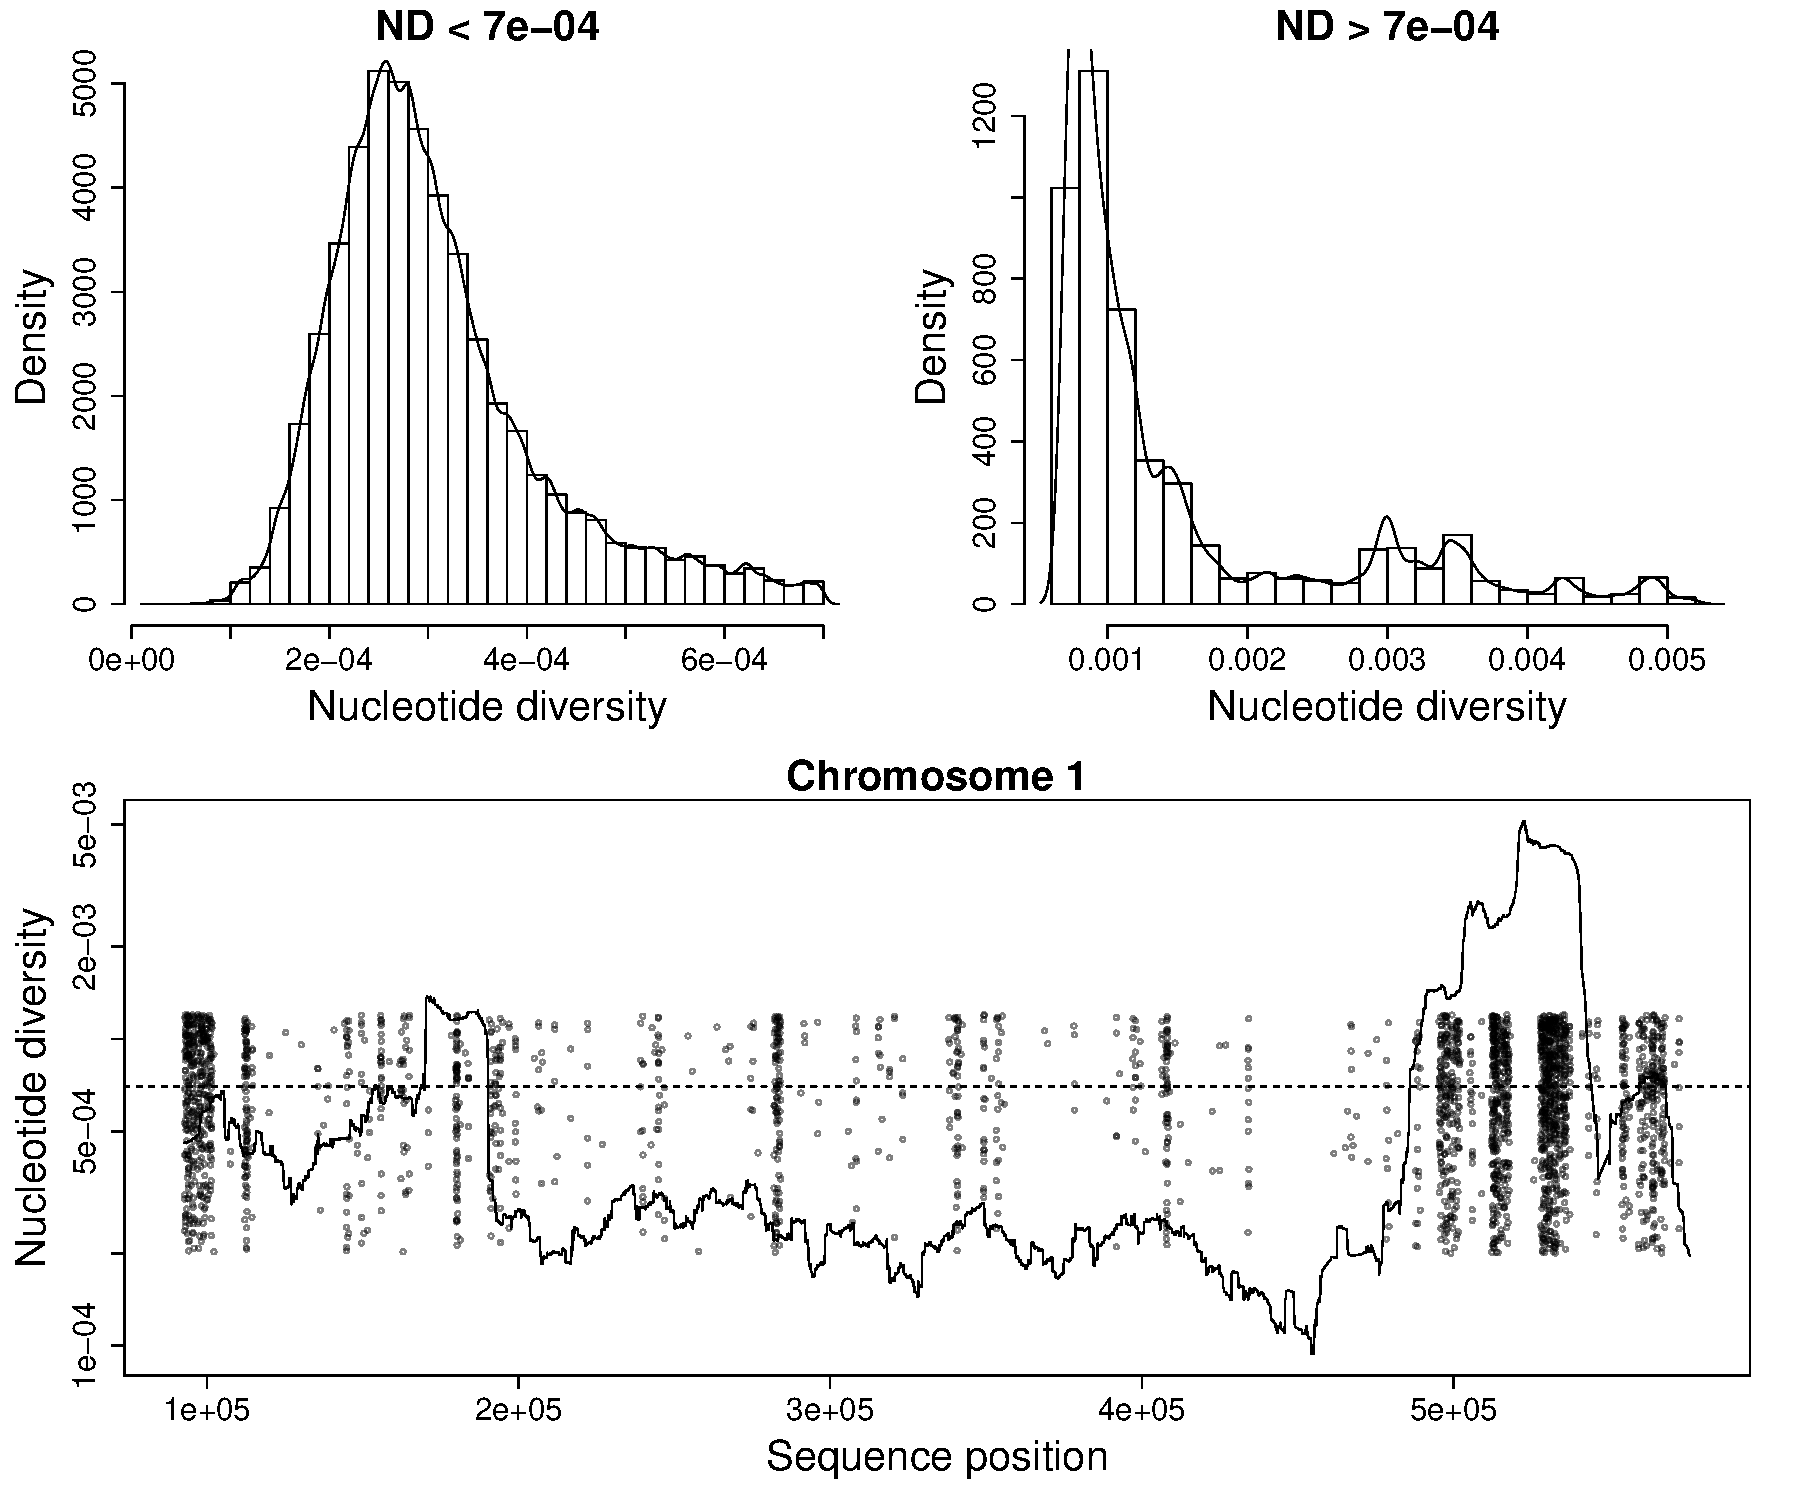
\includegraphics[width=0.7\textwidth]{{supFigures/nd_hist.pdf}}
  \caption{Nucleotide diversity with window size of 20,000. Top two histogram show the heavy tail of ND beyond 0.0007. Bottom figure show ND along {\it P. falciparum} chromosome 1. Scattered Points mark chromosome positions of poorly genotyped SNPs which we exclude from the deconvolution process. These points are jitterred around 0.0007 of visualization.
  }
  \label{fig:nd}
\end{figure}



\subsection{Analysis preparation}
In order to improve the accuracy of the deconvolution process and improve efficiency, we first split the  data into groups, based on genetic similarity. We compute genetic distances between two samples following:
\begin{equation}
d(x, y) = \sum_{l}^{L}\textrm{WSAF}_{x,l} * (1-\textrm{WSAF}_{y,l}) + \textrm{WSAF}_{x,l} * (1-\textrm{WSAF}_{y,l})
\end{equation}
where $l$ represents an arbitrary locus, $L$ denotes the total number of loci, and $\textrm{WSAF}_{s,l}$ indicates the non-reference within-sample allele frequency for sample $s$ at locus $l$. $\textrm{WSAF}_{s,l}$ is then given by $\textrm{WSAF}_{s,l} = \frac{a_{s,l}}{r_{s,l}+a_{s,l}}$ where $a_{s,l}$ is the number of read counts supporting the alternative allele in sample $s$ at locus $l$, and $r_{s,l}$ is the number of read counts supporting the reference allele in sample $s$ at locus $l$.

We find that samples from the same geographical region differentiate into clear clusters. We use this initial grouping as the base for defining the reference panels that assist the deconvolution procedure. Our definition of geographical groups are as follows. In order to reduce the computational time, we restrict to polymorphic sites in each population group:
\begin{enumerate}
  \item Malawi, Congo, with 349,243 sites.
  \item Ghana (Kassena), with 508,607 sites.
  \item Nigeria, Senegal, Mali, with 210,820 sites.
  \item The Gambia, Guinea, Ghana (Kintampo), with 250,828 sites.
  \item Cambodia (Pursat), Cambodia (Pailin), Thailand (Sisakhet), with 44,318 sites.
  \item Vietnam, Laos, Cambodia (Ratanakiri), Cambodia (Preah Vihear), with 88,411 sites.
  \item Bangladesh, Myanmar, Thailand (Mae Sot), Thailand (Ranong), with 84,869 sites.
\end{enumerate}


%\begin{figure}[htp]
  %\centering{}
  %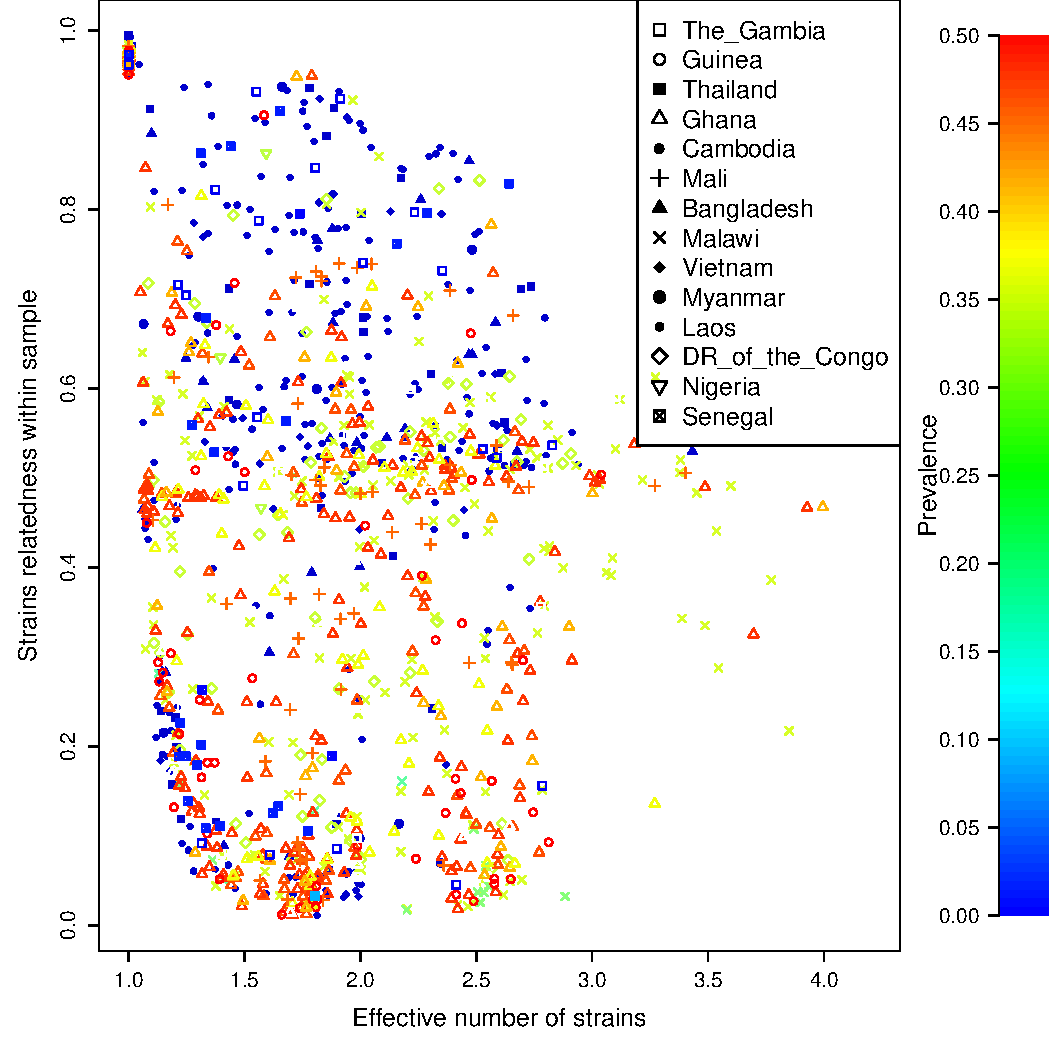
\includegraphics[width=0.8\textwidth]{effK_IBD_colored.pdf}
  %\caption{}\label{fig:tmp1}
%\end{figure}



%\begin{figure}[htp]
  %\centering{}
  %\includegraphics[width=0.8\textwidth]{{llkDiff_vs_eff_k_diff.ibd}.png}
  %\\
  %\includegraphics[width=0.8\textwidth]{{llkDiff_vs_eff_k_diff}.png}
  %\caption{}\label{fig:tmp2}
%\end{figure}


\subsection{Haplotype quality assessment}

We noticed that DEploid-IBD produced chimeric haplotypes when faced with difficult mixtures. For instance, mixed infections in which the co-existing strains have the same relative proportion (e.g. $k=4$ with each strain having a proportion of 25\%), or samples in which proportions are very unbalanced (e.g. k=2 with the marginal strain at 2\%). These artefactual haplotypes show a significant deficit or excess of alternative calls that cannot be explained in terms of their genetic relationship to the reference genome used for mapping and assembly (3D7). To discard problematic haplotypes, we devised a stringent filtering strategy based on $z$-scores. For each population, we computed the distribution of alternative calls observed within the subset of clonal samples ($k=1$). Using this distribution as reference, we computed a $z$-score for each haplotype in a population following

$$z_i = \frac{a_i - \bar{a_r}}{\sigma_r},$$ where $a_i$ denotes the number of alternative calls in the haplotype $i$, and $\bar{a}_r$ and $\sigma_r$ are, respectively, the mean and standard deviation of observed alternative calls in the clonal set of samples from the population of origin. We only retain haplotypes with a $z$-score in the range $(-3,3)$, thus discarding any strain that is three or more standard deviations away, in terms of alternative calls, from the mean observed for clonal samples. By using the set of clonal samples as the reference distribution, we approximate the number of alternative calls expected in a genome belonging to that population. Supp. Figure \ref{fig:ghana-filtering} shows an example of this filtering process for the most problematic population in the dataset (Ghana). Supp. Table \ref{table:haps-discarded-by-country} lists the number of haplotypes discarded by population while Supp. Table \ref{table:haps-discarded-by-COI} describes the number of haplotypes discarded by COI level.


\begin{figure}[ht]
  \centering
    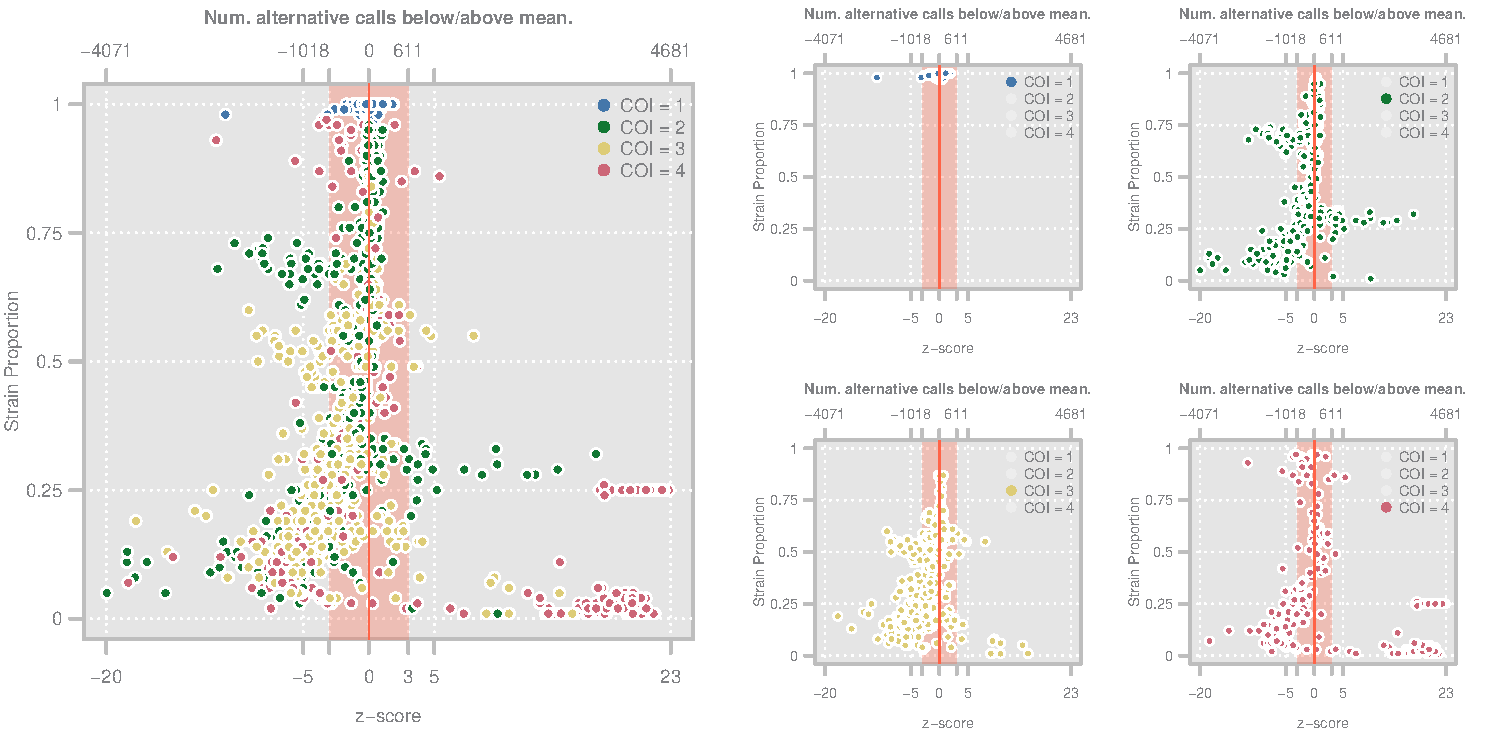
\includegraphics[width=1\textwidth]{figures/qualityGhana.pdf}
  \caption{Diagnostic plots showing the distribution of haplotype quality ($z$-scores) for the Ghanian samples. Left. Scatterplot showing the relationship between haplotype $z$-score and strain proportion. The top axis shows the number of alternative calls below/above the mean of the subset of clonal samples that correspond to a given $z$-score. The vertical red line denotes a $z$-score of $0$ whereas the red-shaded area indicate the haplotypes we retain Point colors show the COI level of the sample. Right. Four views of the same plot in which the samples have been highlighted according to their COI level.}
    \label{fig:ghana-filtering}
\end{figure}



\begin{table}[ht]
\centering
\begin{tabular}{r|r|r|r}
\textbf{Country}  & \textbf{Discarded} & \textbf{Retained} &\textbf{Fraction Discarded} \\
\hline
Bangladesh & 25 & 70 & 0.26 \\
Cambodia & 107 & 704 & 0.14 \\
DR. of Congo & 69 & 155 & 0.31 \\
Ghana & 520 & 615 & 0.46 \\
Guinea & 82 & 88 & 0.48 \\
Laos & 28 & 111 & 0.20 \\
Malawi & 235 & 341 & 0.41 \\
Mali & 40 & 140 & 0.22 \\
Myanmar & 7 & 74 & 0.09 \\
Senegal & 2 & 167 & 0.01\\
Thailand & 28 & 170 & 0.14 \\
The Gambia & 22 & 73 & 0.23 \\
Vietnam & 23 & 118 & 0.16\\
\hline
\textbf{Total} & 1194 & 2826 & 0.30
\end{tabular}
\vspace{.2cm}
\caption{Number of haplotypes discarded and retained for each population in the Pf3k dataset.}
\label{table:haps-discarded-by-country}
\end{table}


\begin{table}[ht]
\centering
\begin{tabular}{r|r|r|r}
\textbf{COI}  & \textbf{Retained} & \textbf{Discarded} & \textbf{Fraction Discarded} \\
\hline
1 & 1312 & 33 & 0.02 \\
2 & 670 & 280 & 0.29 \\
3 & 585 & 528 & 0.47 \\
4 & 259 & 353 & 0.57 \\
\hline
\textbf{Total} & 2826 & 1194 &  \\
\hline
\textbf{Fraction} & 0.70 & 0.30 & \\
\end{tabular}
\vspace{.2cm}
\caption{Number of haplotypes retained and discarded stratified by COI level.}
\label{table:haps-discarded-by-COI}
\end{table}


\subsection{Combining clonal sample pairs for background IBD computation}
In order to construct the background IBD profile for classification, we combine clonal sample pairs to create artificial mixture at each sampling site to study the background IBD distribution. We assume artificial mixtures mimic infections from independent mosquito bites. The strain relative abundance is proportional to the median of sequence depth. The artificial mixture sample coverage is then obtained by accumulating the reference and alternative allele counts of two clonal samples. Similar to {\tt DEploidIBD} deconvolution, high allele count SNPs causes high leverage in the model. By combining allele counts from two samples, it creates artificial high leverage SNPs again. In addition, the sample sequence depth and skewness are heterogeneous due to different sample preparation and sequencing protocols. We reduce the {\tt DEploidIBD} filtering threshold from 99.5\% to 80\%, and use low recombination probabilities to avoid false IBD break detections. We validate our method using lab crosses \citep{Miles2016}, and compare the IBD block detections using \citet{Li2003}'s painting with parental strains and {\tt DEploidIBD} algorithm (Figure~\ref{fig:bgibd}).


\begin{figure}[ht]
  \centering{}
  %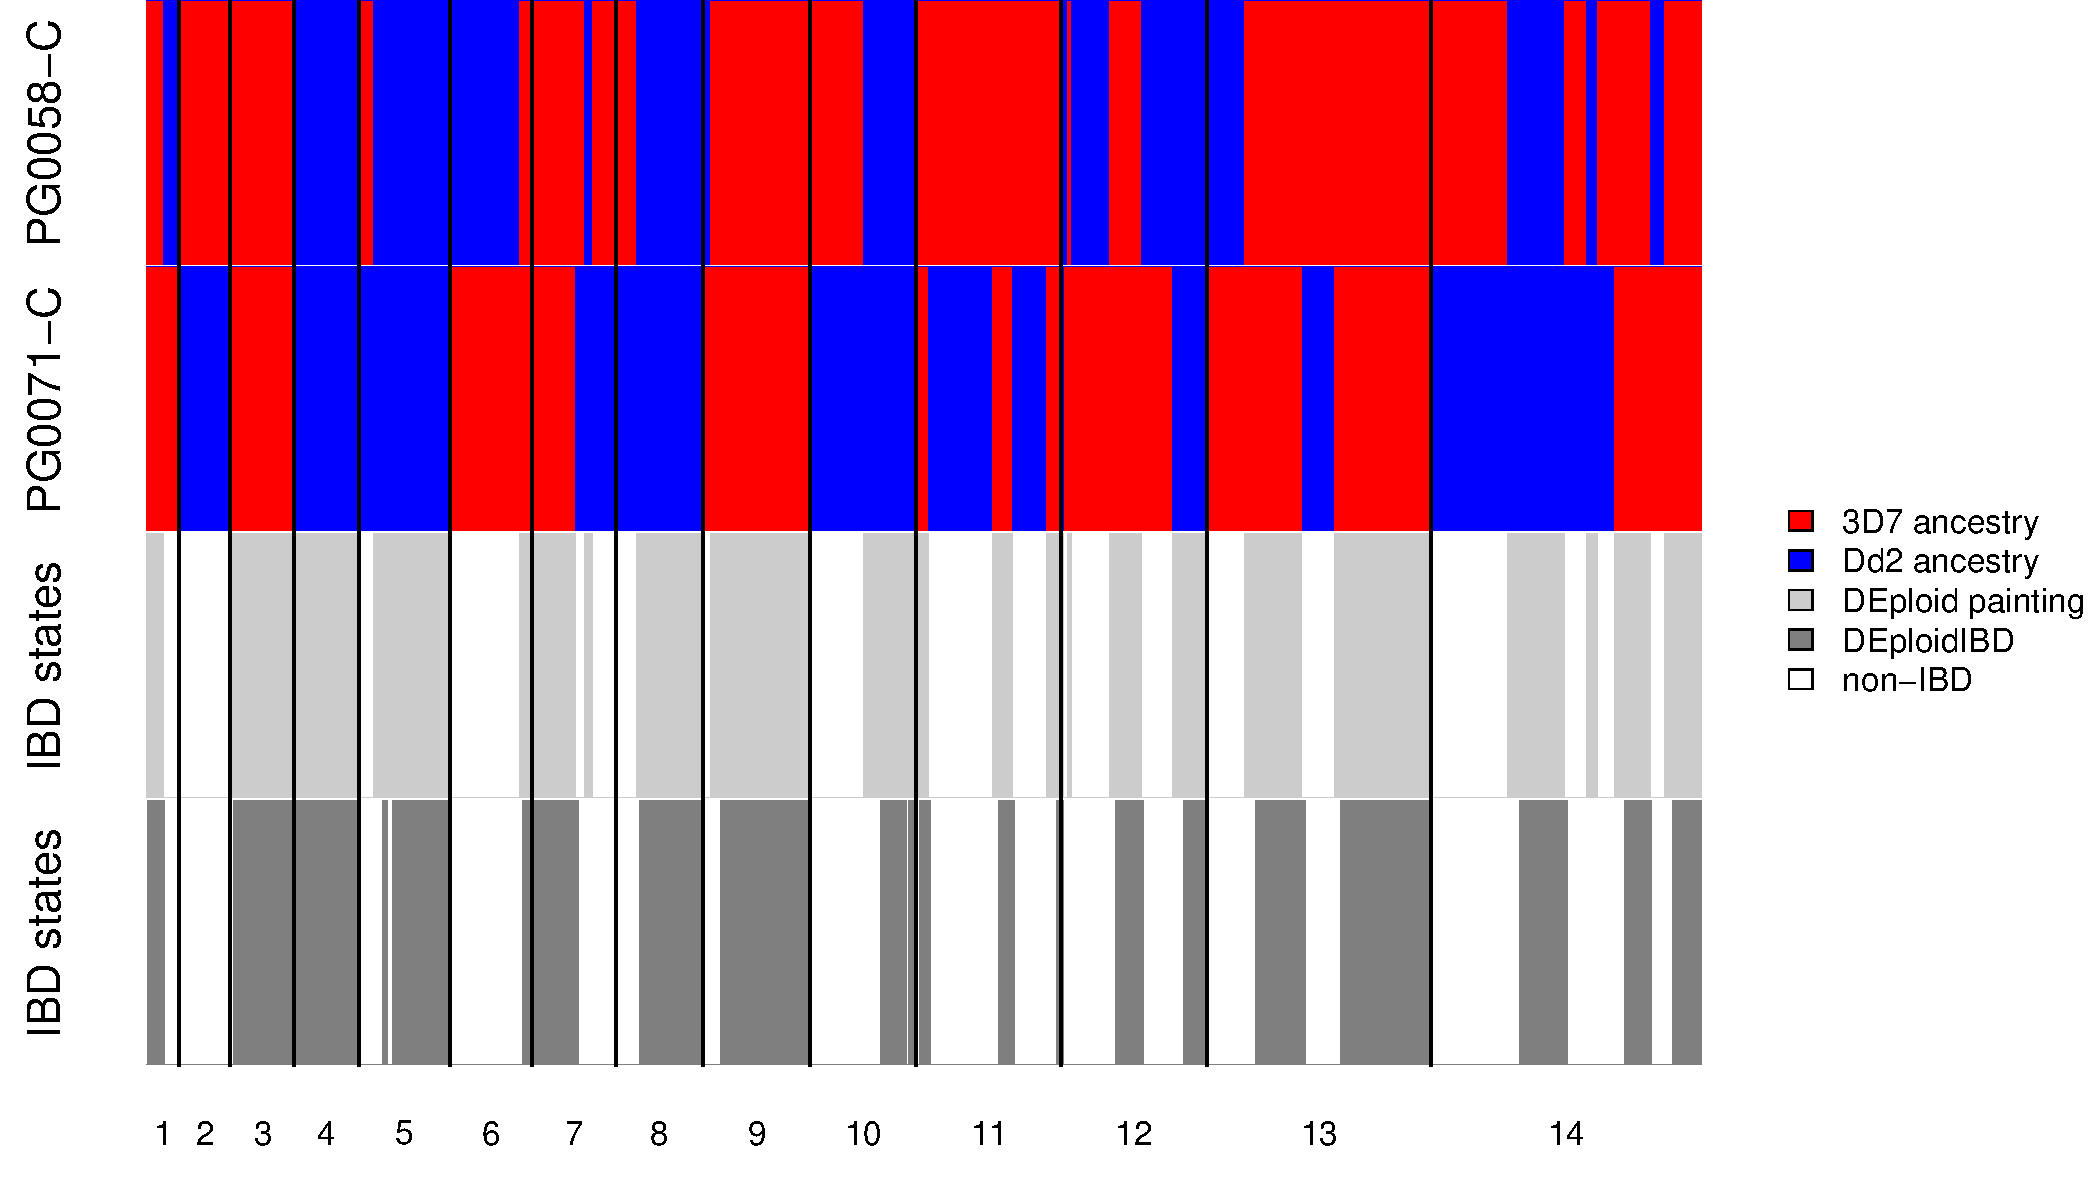
\includegraphics[width = .85\textwidth]{bgIBDvalidation/bgIBD.pdf}
  \subfloat[]{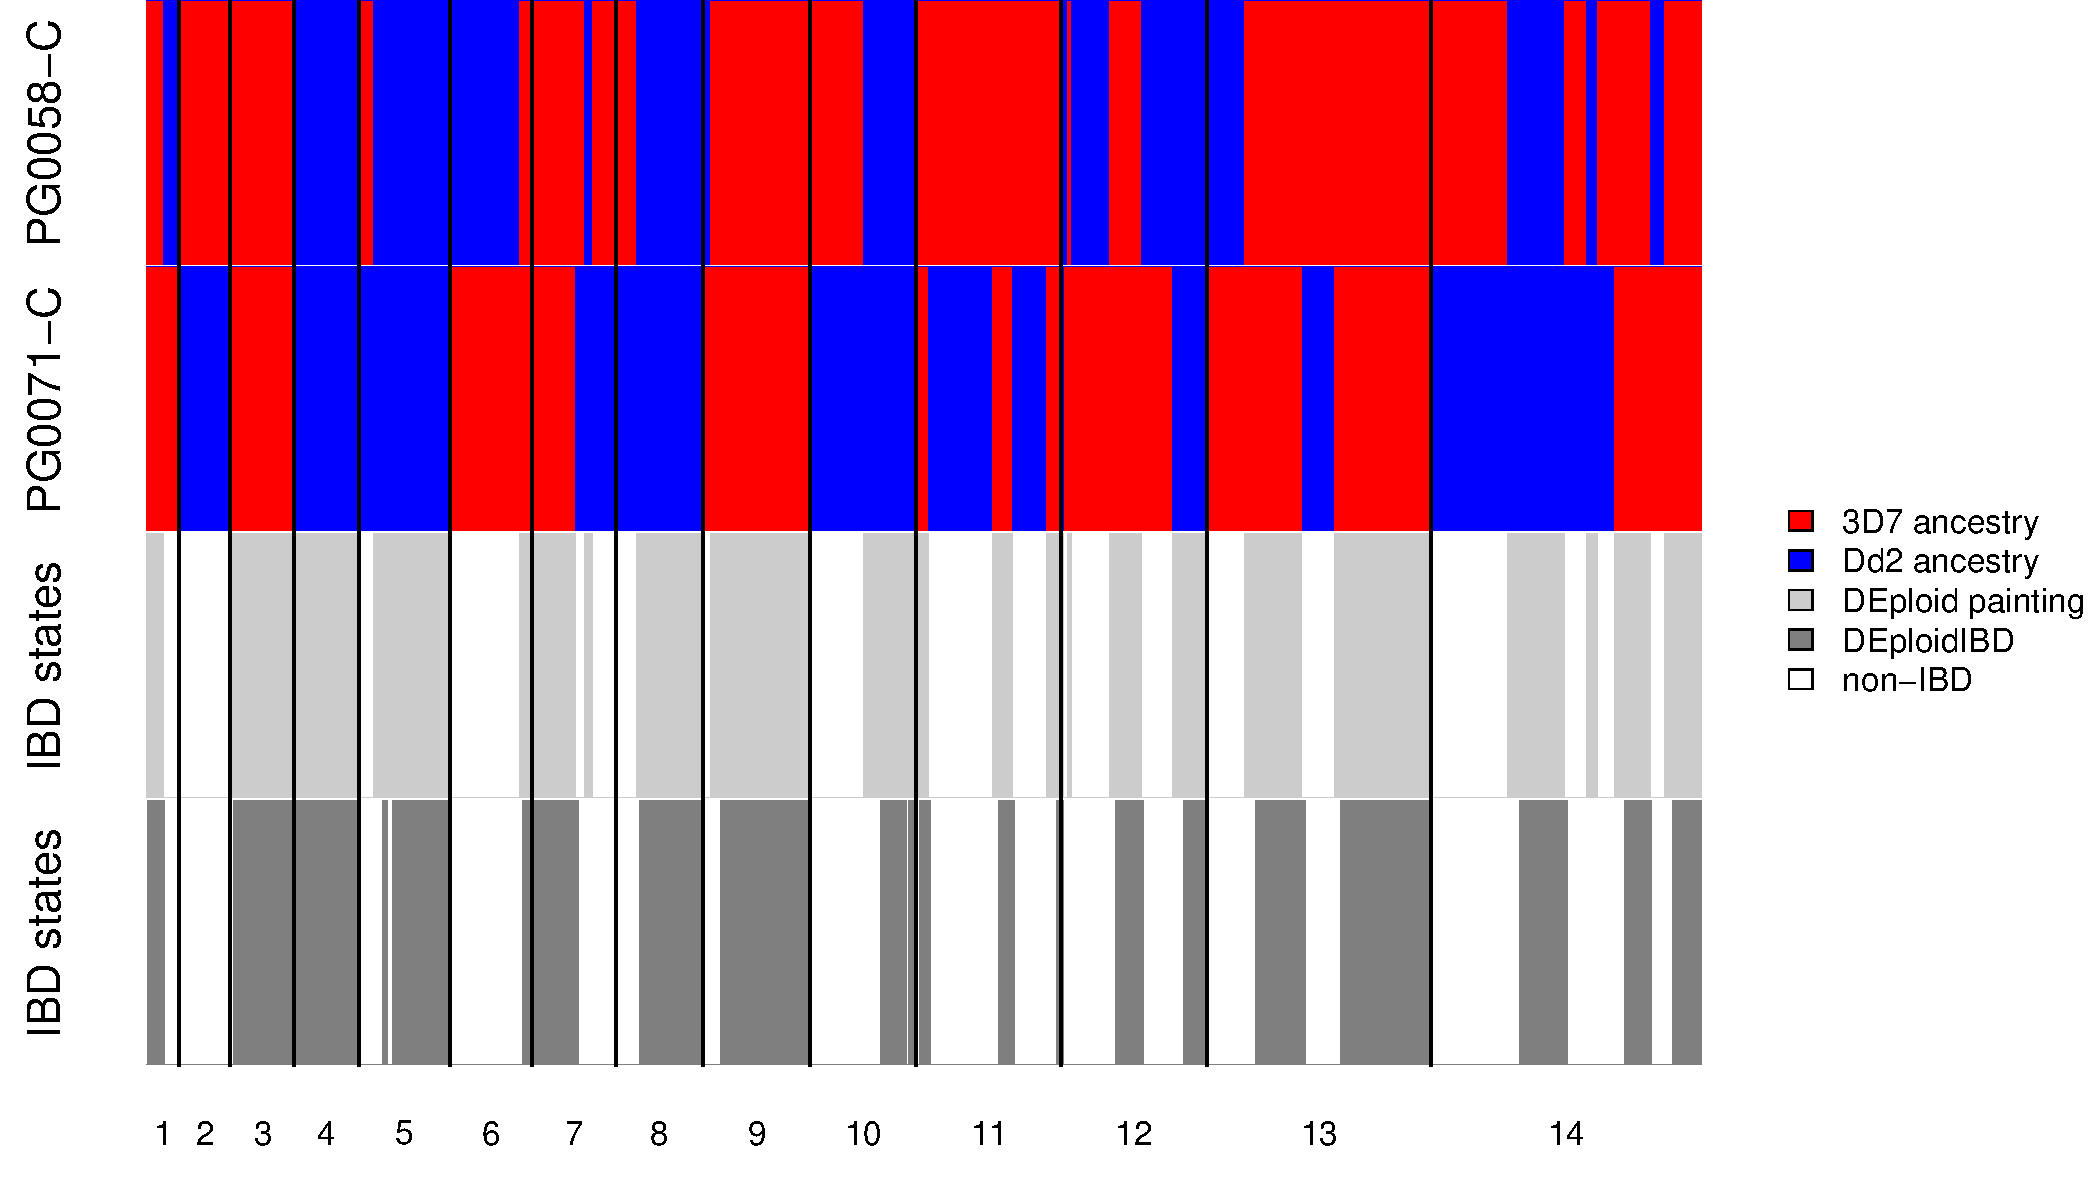
\includegraphics[width = .65\textwidth]{bgIBDvalidation/bgIBD.pdf}}
  \subfloat[]{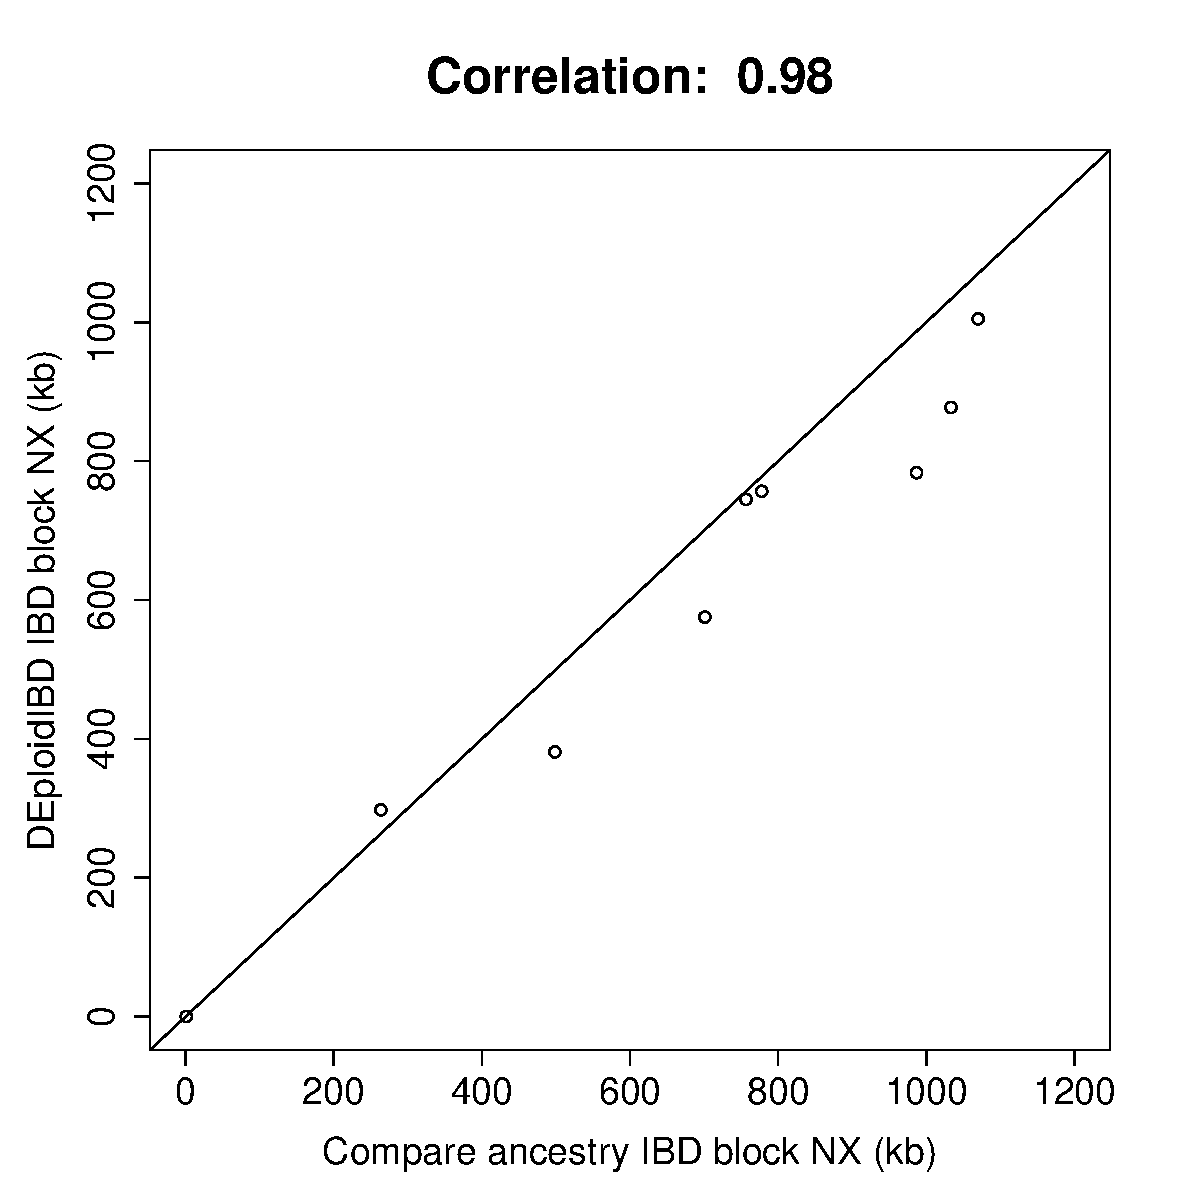
\includegraphics[width = .35\textwidth]{bgIBDvalidation/bgN50.pdf}}
  %\subfloat[]{\includegraphics[width = .85\textwidth]{bgIBDvalidation/IBDtracklengthVsPercentage_data_clean.pdf}}
  \caption{(A) Comparison of IBD block detection of {\tt DEploidIBD} using artificial mixtures of lab crosses PG0071-C and PG0058-C (last track) with IBD block detection from ancestral state inference from \citet{Li2003}. (B) Scatter plot of IBD segment Nx values extracted by comparing clonal sample ancestry and using {\tt DEploidIBD} on artificial mixtures.}\label{fig:bgibd}
\end{figure}

\newpage
\FloatBarrier
\section{Expected levels of IBD in \textit{ P.falciparum } mixed infections}

The amount of IBD observed in a mixed infection is a function of the number of oocysts present in the biting mosquito. We will demonstrate this below.

First, let us briefly review the fundamentals of malaria meiosis. In our case, we imagine a mosquito bites a human host containing two distinct malaria strains, namely $A$ and $B$. Some number of gametocytes of $A$ and $B$ are imbibed during the bite, differentiate into gametes, and undergo fertilization to produce zygotes. Some fraction of these zygotes succeed in establishing themselves as oocysts on the mosquito midgut. Three fertilization outcomes are possible: $A+A$ or $B+B$ (inbred oocysts, $n_{ii}$), or $A+B$ (outbred oocysts, $n_{ij}$). The oocyst state of a mosquito can be characterized by ($n_{ij}$, $n_{ii}$). Which strain is maternal and paternal may vary from oocyst to oocyst, but this is of no consequence here.

A $k=2$ mixed infection is established when two distinct sporozoites, produced from the oocysts of this mosquito, infect a host. Each oocyst produces thousands of sporozoites, of four types, which pool in the mosquito salivary glands. Imagine drawing a $k=2$ mixed infection from a mosquito harbouring a single outbred oocyst ($n_{ij}$~=~1). In such a mosquito there are two copies of each of the two strains (two sets of sister chromatids; $A$,~$A$,~$B$,~$B$). We first consider zero recombination: There are two possible pairs with IBD fraction 1s. Assuming parental strains are unrelated, the remaining ${4 \choose 2}$ pairs will have an IBD of 0. Thus a single $n_{ij}$ oocyst has an expected IBD of $E[f]= 2/{4 \choose 2} = 1/3$. We draw pairs without replacement, because if sporozoites of only one type seed the infection, it will be $k=1$. Assuming free recombination, it shuffles how the total identity is distributed between pairs, without destroying any identity (identity is created by DNA replication and destroyed by mutation); the expectation is taken over all pairs and is thus unaffected.

Computing the expected IBD fraction for a mosquito posessing $n_{ij}$ outbred oocysts is an extension of the above. Again ignoring recombination, the expected IBD fraction $E[f|n_{ij}]$ is equal to the total number of pairs with an IBD of 1 (IBD pairs), over all possible pairs. In a mosquito with $n_{ij}$ oocysts, we have $2n_{ij}$ copies of each parental strain, thus we have ${2n_{ij} \choose 2}$ IBD pairs for each parental strain, thus $2 {2n_{ij} \choose 2}$ IBD pairs total. Dividing this by the total number of pairs amongst $n_{ij}$ oocysts we have...

\begin{equation} \label{eq1}
E[f|n_{ij} > 0] = \frac{2{2n_{ij} \choose 2}}{{4n_{ij} \choose 2}} = \frac{2n_{ij} - 1}{4n_{ij} - 1}
\end{equation}

The above yields $1/3$ for $n_{ij}=1$, approaching $1/2$ as $n_{ij}$ grows. It has been validated with \texttt{pf-meiosis} in Figure~\ref{fig:validoocyst}.


\begin{figure}[pt]
  \centering{}
  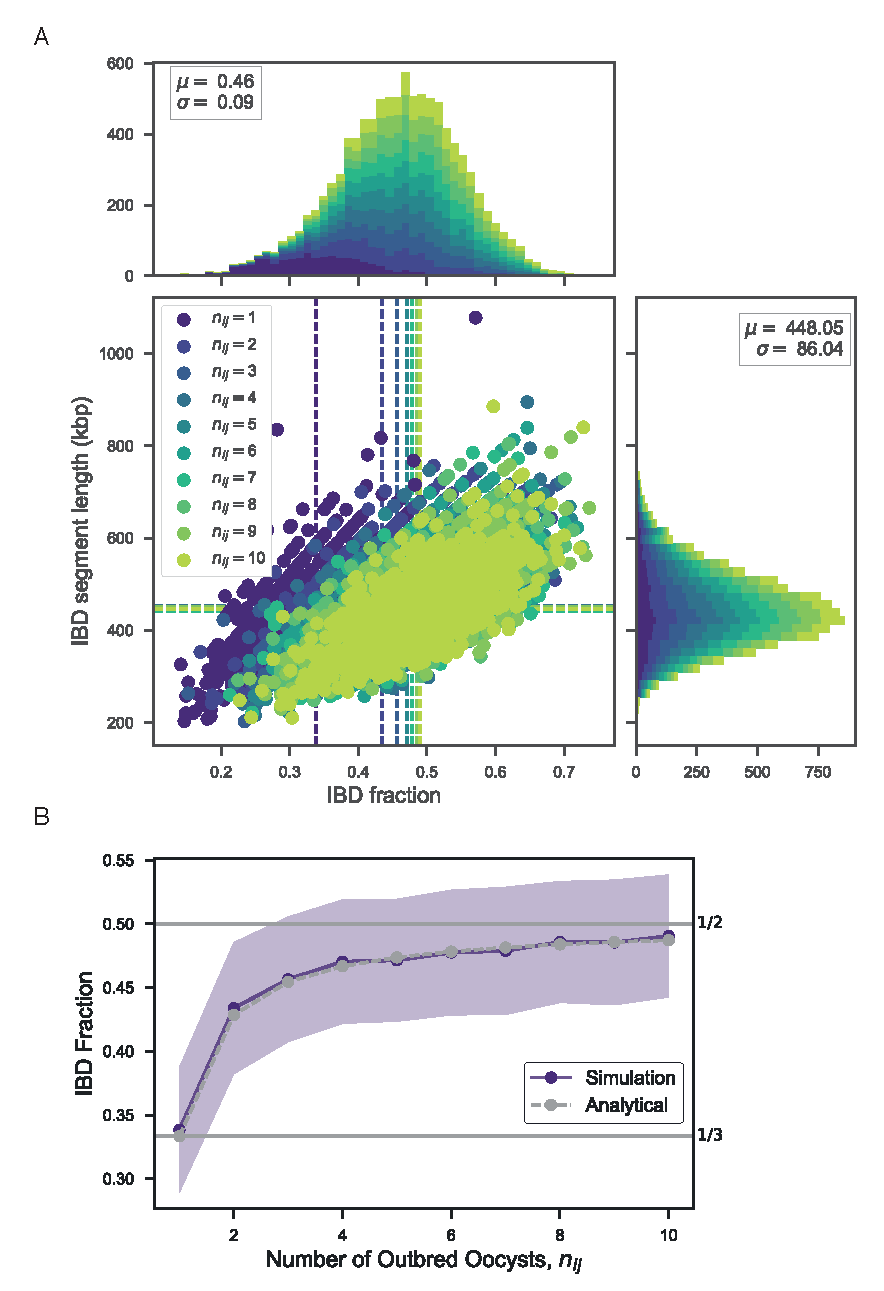
\includegraphics[width = .85\textwidth]{supFigures/supp-Fig1.pdf}
  \caption{Exploring the relationship between number of outbred oocysts ($n_{ij}$) and IBD. (A) Joint IBD fraction and IBD segment length distributions for $k=2$ mixed infections simulated from two unrelated strains and a fixed number of outbred oocysts $n_{ij}$, using \texttt{pf-meiosis}. Mean values for each distribution are indicated by same-color dashed lines. Each distribution is created from 1000 simulated mixed infections. (B) Validation of theoretical result given in text (S1.8). Line plot compares trend in expected IBD fraction with the number of outbred oocysts, $n_{ij}$, for infections simulated in panel A, and the analytical expression S1.8.} \label{fig:validoocyst}
\end{figure}

Including $n_{ii}$ oocysts is somewhat complicating, as some pairs (selected without replacement) may be identical (thus yielding $k=1$) or completely unrelated (yielding $k=2$, but effectively without having undergone meiosis or producing any detectable recombination breakpoints between parental strains).  We are interested in the expected IBD produced as a result of meiosis between parental strains, and thus for the moment we exclude these pairs. In practice, this means the mosquito must have at least one outbred oocyst, and at least one of the infecting sporozoites must be from an outbred oocyst.

The derivation is as above: first ignoring recombination and segregation, then enumerating all IBD pairs (pairs with IBD fraction of 1) and dividing by the total number of pairs to compute the expectation. Note that the additional IBD pairs possible between an outbred and inbred oocyst are given by the term $8n_{ij}n_{ii}$, and that you can no longer use all possible pairs drawn without replacement as the denominator, but must exclude the pairs described above.

\begin{align}
E[f|n_{ij} > 0, n_{ii}] & = \frac{2{2n_{ij} \choose 2} + 8n_{ij}n_{ii}}{2{2n_{ij} \choose 2} + 16n_{ij}n_{ii} + 4n_{ij}^2} \nonumber\\
& = \frac{{2n_{ij} \choose 2} + 4n_{ij}n_{ii}}{{2n_{ij} \choose 2} + 8n_{ij}n_{ii} + 2n_{ij}^2} \nonumber\\
& = \frac{n_{ij}(2n_{ij} - 1) + 4n_{ij}n_{ii}}{n_{ij}(2n_{ij} - 1) + 8n_{ij}n_{ii} + 2n_{ij}^2} \nonumber\\
& = \frac{2n_{ij} - 1 + 4n_{ii}}{2n_{ij} - 1 + 8n_{ii} + 2n_{ij}} \nonumber\\
& = \frac{2(n_{ij} + 2n_{ii}) - 1}{4(n_{ij} + 2n_{ii}) - 1}  \label{eq2}
\end{align}


Which is of a similar form to above, but increases to $1/2$ quicker if more inbred oocysts are present. As before the equation is validated in Figure~\ref{fig:validinbred}A.

\begin{figure}[ht]
  \centering{}
  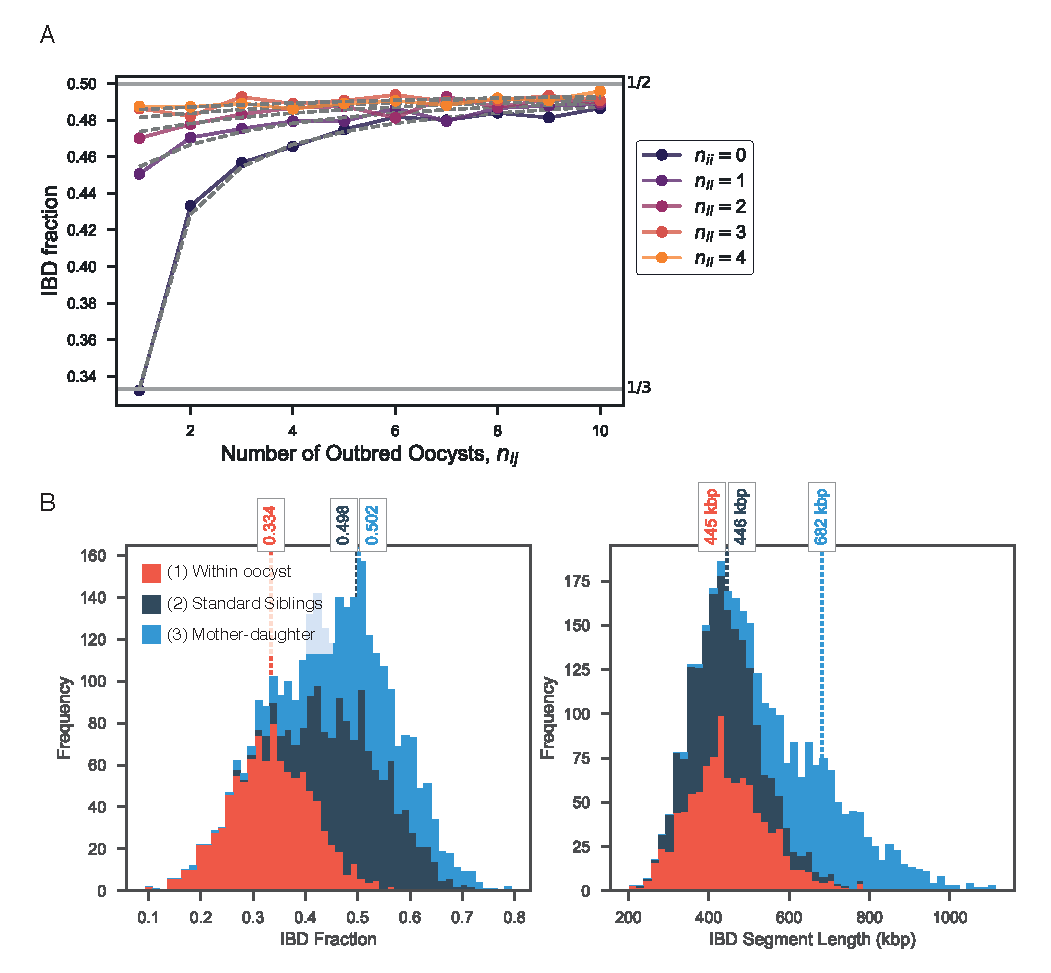
\includegraphics[width = .85\textwidth]{supFigures/supp-Fig2.pdf}
  \caption{Exploring expected IBD allowing for outbred ($n_{ij}$) and inbred ($n_{ii}$) (A) Validation of theoretical result given in text (S1.9). Line plot compares trend in expected IBD fraction with the number of outbred oocysts, $n_{ij}$, for infections simulated in panel A, and the analytical expression S1.9. Differing number of inbred oocysts are indicated with color. (B) The three types of pairs. } \label{fig:validinbred}
\end{figure}

The expression for $E[f|n_{ij} > 0, n_{ii}]$ can also be derived by recognizing that there are three \textit{types} of pairs possible in a mosquito with a collection of $n_{ij}$ and $n_{ii}$ oocysts: (1) a pair can contain two strains from a single $n_{ij}$, ($n^{o=1}_{ij}$); (2) a pair can contain two strains from two different $n_{ij}$, ($n^{o=2}_{ij}$); or (3) a pair can contain one strain from an $n_{ij}$ oocyst and one from an $n_{ii}$ oocyst, $n^{o=2}_{ij, ii}$. Pair type (1) is unique to malaria and has an  $E[f|n^{o=1}_{ij}]=1/3$, as shown above; pair type (2) are standard siblings with $E[f|n^{o=2}_{ij}]=1/2$; and pair type (3) represent a mother-daughter relationship, also with $E[f|n^{o=2}_{ij, ii}]=1/2$. The full IBD fraction and IBD segment length distributions of these pairs were generated using \texttt{pf-meiosis} and can be seen in Figure~\ref{fig:validinbred}B. We enumerate the number of each pair type given $n_{ij}$ and $n_{ii}$, weighted by their expectation, to derive $E[f|n_{ij} > 0, n_{ii}]$:


\begin{align}
E[f|n_{ij} > 0, n_{ii}] & = \frac{n^{o=1}_{ij}E[f|n^{o=1}_{ij}] + n^{o=2}_{ij}E[f|n^{o=2}_{ij}]
+ n^{o=2}_{ij, ii}E[f|n^{o=2}_{ij, ii}]}{n^{o=1}_{ij} + n^{o=2}_{ij} + n^{o=2}_{ij, ii}} \nonumber\\
& = \frac{ n_{ij}{4\choose 2}1/3 + 16{n_{ij}\choose 2}1/2 + 16n_{ij}n_{ii}1/2}{
n_{ij}{4\choose 2} + 16{n_{ij}\choose 2} + 16n_{ij}n_{ii}} \nonumber\\
& = \frac{2n_{ij} + 4n_{ij}(n_{ij} - 1) + 8n_{ij}n_{ii}}{6n_{ij} + 8n_{ij}(n_{ij} - 1) + 16n_{ij}n_{ii}}\nonumber\\
& = \frac{1 + 2(n_{ij} - 1) + 4n_{ii}}{3 + 4(n_{ij} - 1) + 8n_{ii}} \nonumber\\
& = \frac{2(n_{ij} + 2n_{ii}) - 1}{4(n_{ij} + 2n_{ii}) - 1}
\end{align}
As above.

\FloatBarrier

\bibliography{mixedIBD.bib}

\end{document}
